\chapter{Fundamentals}
\label{chapter:fundamental}
In this first chapter, we lay out the fundamentals used in the rest of this thesis. At the beginning, we will introduce basic definitions such as \emph{utterance}, \emph{sample} and \emph{conversation}. We will then follow up with an introduction into machine learning using a special variant of \emph{Neural Networks} (NN), called \emph{Recurrent Neural Network} (RNN). We show the basic principles behind it and explain problems this RNNs have in practice, and how the can be solved by utilizing other forms of RNNs. We then show how RNNs can be used to build models, called \emph{Sequence-To-Sequence} (seq2seq) models \cite{Sutskever:2014}, which are capable of learning and using a language in a conversational context.

The following introduction only covers a small part of the spectrum of possibilities with regard to the tasks these models can perform. Basically, we are restricting our explanations to the supervised learning use-case and ignore the unsupervised ones, even though they have a wide area of applications (e.g. dimensionality reduction, regression) as shown by !REFERENZ FÜR UNSUPERVISED LEARNING?!. A basic introduction into the principles of neural networks can be found in appendix \ref{fundamentals:neural_networks}.

\section{Definitions}
\paragraph{Utterance} \blindtext
\paragraph{Sample} \blindtext
\paragraph{Conversation} \blindtext

\section{Recurrent Neural Networks}
\emph{Recurrent neural networks} (RNN) are a special variation of the NNs described in appendix \ref{fundamentals:neural_networks}. The main difference between them is, that RNNs have a recurrence built into it, which allows them to adapt to problems which also have a temporal dimension and are dependent on data from differente timesteps to solve. We're also going into the problems such RNNs have due to their recurrence and how this problem can be solved by exploiting another form of RNN, called \emph{Long Short-Term Memory Networks} (LSMT).

\paragraph{RNNs in principle}
One of the main restrictions of vanilla NNs is the following: Assume a task, where the NN is conditioned to output a prediction on tomorrows weather given yesterdays. Now, if one would use a vanilla NN as described in the appendix, the main restriction would be that the NN has to make its prediction solely based on the weather information of the day before. Such a model does not take into account, that weather is not only dependent on the weather of the previous day, but also on the days before. This could be solved by feeding, say, the weather of the last week to the network instead of just the weather of the previous day. But if new scientific evident now shows, that weather is not only dependent on last week, but also on the last month, probably the last year, we quickly get into problems due to the sheer size of a NN performing such tasks, because the input size grows rapidly. Also, such a NN would still be static in the way, that one cannot simply change the time-window used to feed to the network. If one settles with one month, it will always be able predict the weather based on the last month, but not any different time-window, otherwise the NN has to be retrained using another time-window in order to work again as before. RNNs (see figure \ref{fundamentals:rnn:rolled_vanilla}) try to solve this problem by introducing a recurrence into the network, which allows it to exploit informations not only from the current input, but also from inputs of the past. In a more formal way, one could say that this recurrence allows RNNs to ''exhibit dynamic behaviour across the temporal dimension of the input data''.

\begin{figure}[h]
	\label{fundamentals:rnn:rolled_vanilla}
	\centering
	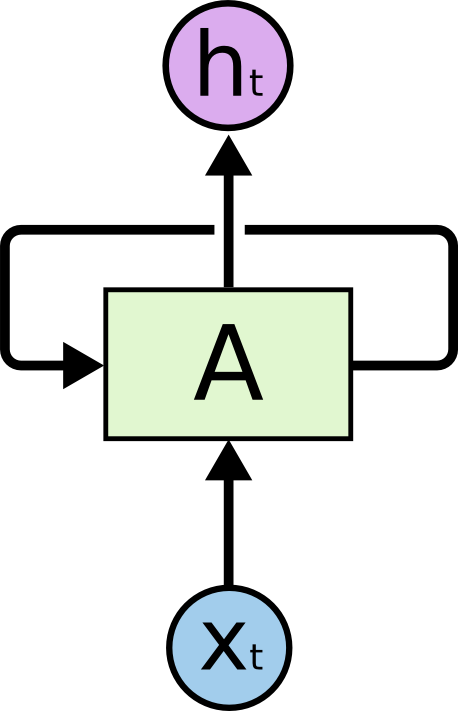
\includegraphics[width=5cm]{img/rnn_rolled}
	\caption{Basic layout of an RNN.\protect\footnotemark}
\end{figure}
\footnotetext{http://colah.github.io/posts/2015-08-Understanding-LSTMs/}

Before explaining how this recurrence can be used to solve the weather prediction problem, let's first show the equations used for the forwared propagation in an RNN. This equations assume, that the inner part of the RNN consists of three distinct layers, called input, hidden and output layer. The internal structure is similar to the one of NNs, as explained in appendix \ref{fundamentals:neural_network}.

\begin{equation}
\begin{split}
o_t  & =  \varphi(\mathbf{w} \cdot \mathbf{x}_t + \mathbf{u} \cdot \mathbf{h}_{t-1}) \\
& = \varphi\bigg(\sum_{i=0}^{n} w_i x_{ti} + \sum_{i=0}^{n} u_i h_{t-1i}\bigg)
\end{split}
\label{fundamentals:rnn:forward_equation:hidden}
\end{equation}


\begin{equation}
\begin{split}
h_t  & =  \varphi(\mathbf{w} \cdot \mathbf{x}_t + \mathbf{u} \cdot \mathbf{h}_{t-1}) \\
     & = \varphi\bigg(\sum_{i=0}^{n} w_i x_{ti} + \sum_{i=0}^{n} u_i h_{t-1i}\bigg)
\end{split}
\label{fundamentals:rnn:forward_equation:output}
\end{equation}

In the equations above, one can see different variables with different indices which we'll explain briefly:

\begin{itemize}[noitemsep]
	\item $x_t$ stands for the input at timestep $t$.
	\item $o_t$ stands for the output of the network at timestep $t$.
	\item $h_t$ stands for the output of the hidden layer before applying the activation function.
	\item $\mathbf{w}$ and $\mathbf{u}$ stand for the weight matrices which are learnt while training.
	\item $\varphi$ is the activation function to be used on the output of the neurons in the hidden layer.
\end{itemize}

\paragraph{Vanishing / Exploding Gradient Problem}
\begin{itemize}
	\item Problem RNNs face in practice
	\item Explain unrolling briefly
	\item Explain gradient descent with TBTT
	\item Show how the identity function on the recurrence can solve this problem.
	\item Reference formal proofs for the problem (with links to dynamical systems).
\end{itemize}

\paragraph{Long Short-Term Memory Networks}
\begin{itemize}
	\item Show basic structure with gates.
	\item Explain that identity function solve the vanishing/exploding gradient problem.
	\item Explain gradient descent with TBTT
	\item Show how the identity function on the recurrence can solve this problem.
	\item Adapt weather prediction problem to LSTM.
\end{itemize}

\section{Sequence-To-Sequence Learning}
\paragraph{Model} 
\begin{itemize}
	\item Explain basic idea behind model.
	\item Show different tasks which can be solved by using such models..
\end{itemize}

\paragraph{Decoding Approaches}
\begin{itemize}
	\item Explain two approaches: Greedy and Beam-Search.
	\item Explain why greedy might not give satisfactory results.
\end{itemize}
\paragraph{Soft-Attention Mechanism}
\begin{itemize}
	\item Draw link to "human" attention mechanism
	\item Show how this works on a more formal level.
\end{itemize}

\section{Technischer Aufbau}
\label{technical_setup}
Im folgenden Abschnitt wird der technische Aufbau erläutert, welcher verwendet wird, um die in Kapitel \ref{sec:Experimente_Resultate} beschriebenen Experimente durchzuführen. Eine Beschreibung zur Verwendung des Systems befindet sich in Anhang \ref{appendix:software_usage}.

\paragraph{Vorarbeiten}
\label{technichal_setup:prework}
Der Grundaufbau der verwendeten Software wurde vom InIT mithilfe von \texttt{keras}\footnote{https://keras.io/} implementiert und zur Durchführung dieser Arbeit zur Verfügung gestellt. Im Rahmen dieses Grundaufbaus wurden die folgenden Funktionalitäten bereits implementiert:

\begin{itemize}[noitemsep]
	\item Implementation des CNN in \texttt{keras} und verwendung von \texttt{theano} \cite{theanoCitShort} als Backend für die \gls{GPU}s.
	\item Implementation von Evaluations-Metriken.
	\item Skripte mit den folgenden Funktionalitäten: Trainieren des CNN, Laden von TSV Dateien, Vorverarbeiten von Word-Embeddings.
\end{itemize}

\paragraph{Anforderungen}
\label{technical_setup:requirements}
Ein zu implementierendes System, mit welchem die Experimente durchgeführt werden können, soll die folgenden Eigenschaften aufweisen:

\begin{itemize}
	\item \textbf{Parametrisierbarkeit}: Dadurch, dass eine grosse Anzahl kleiner Experimente durchgeführt werden muss, soll das System die Möglichkeit bieten, Experimente parametrisiert durchzuführen.
	\item \textbf{Wiederholbarkeit}: Experimente sollen mit einem minimalen Mehraufwand mehrfach durchgeführt werden können.  
	\item \textbf{Übersichtlichkeit}: Resultate der Experimente sollen übersichtlich und einfach zugänglich sein.
	\item \textbf{Auswertbarkeit}: Resultate sollen automatisiert ausgewertet werden können.
\end{itemize}

\paragraph{Funktionalität}
\label{technical_setup:functionality}
Um ein System, welches die oben beschriebenen Anforderungen erfüllt zu erhalten, werden die folgenden Komponenten implementiert:

\begin{itemize}
	\item \textbf{Executor}: Der \emph{Executor} ist zuständig für das Training der CNNs mithilfe von \texttt{keras}. Beim Start akzeptiert er die Konfiguration als Parameter. Das Experiment wird mit dem Laden der benötigten Daten und dem anschliessenden Training des CNN gestartet. Am Ende jeder Epoche wird das aktuelle CNN auf den Validierungsdaten getestet und die konfigurierten Metriken ausgewertet. Diese werden am Ende zusammen mit dem trainierten CNN (Gewichte im HDF5-Format\footnote{https://support.hdfgroup.org/HDF5/}, das CNN Model als JSON) in einen für das Experiment vorgesehenen Ordner gespeichert. Die Metriken werden ebenfalls in dem dafür vorgesehenen Ordner abgespeichert.
	\item \textbf{Config Management}: Experimente werden über Konfigurationen im JSON-Format\footnote{http://www.json.org/} parametrisiert. Über diese Konfiguration können viele wichtige Parameter für die Ausführung festgelegt werden, so zum Beispiel: Anzahl Epochen, Trainings- und Validierungsdaten, Parameter für die k-fold Cross-Validation oder auch bereits trainierte Modelle können geladen werden. Detailierte Erläuterungen zu den einzelnen Parametern können im Anhang \ref{appendix:software_usage} gefunden werden.
	\item \textbf{DataLoader}: Mithilfe des \emph{DataLoader} können Trainings- und Validierungsdaten im TSV\footnote{https://reference.wolfram.com/language/ref/format/TSV.html} Dateiformat geladen werden. Die zu ladenden Daten können dabei aus einer oder mehreren TSV-Dateien stammen. Im Falle, dass mehrere TSV Dateien angegeben werden, kann über die Konfiguration das Verhältnis angegeben werden, in welchem die Daten aus den einzelnen Dateien verschmischt werden sollen.
	\item \textbf{Skripte}: Die Auswertung der einzelnen Experimente geschieht über dafür erstellte Skripte.
	\item \textbf{Weboberfläche}: Auf die Resultate der Experimente kann über eine eigens dafür entwickelte Weboberfläche zugegriffen werden. Ausserdem besteht die Möglichkeit Plots über die Metriken, welche während des Trainings- und Validierungsprozess gesammelt werden, zu erstellen.
	
\end{itemize}
Die oben beschriebenen Komponenten erlauben es, Experimente mittels JSON Konfigurationen zu starten und den gesamten Trainings- und Validierungsprozess mittels Metriken zu überwachen und zu dokumentieren.

\paragraph{Skripte}
\label{technical_setup:scripts}
Für die Durchführung der Experimente wurden diverse Skripte erstellt, um die Handhabung zu vereinfachen und Auswertungen zu ermöglichen. Die Liste der implementierten Scripts umfasst unter anderem die folgenden:

\begin{itemize}[noitemsep]
	\item Erstellen von Plots der Lernkurven und Metriken
	\item Erstellen von Word-Embeddings über einen Text-Corpus
	\item Erstellen von Statistiken zu Trainings- und Validierungsdaten
	\item Vorverarbeitung von Trainingsdaten für die Distant-Phase
	\item Erstellen von Visualisierungen von Word-Embeddings mittels PCA
	\item Diverse Wartungsskripte zur Generierung und Verwaltung von Experimenten
\end{itemize}

\paragraph{Weboberfläche}
\label{technical_setup:webgui}
Um die dritte Anforderung nach Übersichtlichkeit und Auswertbarkeit zu erfüllen, wird eine Weboberfläche umgesetzt, mit welchem die Parameter und Resultate aller durchgeführten Experimente übersichtlich und an einem Ort zur Verfügung gestellt werden. Für die Implementation wird die \texttt{python}\footnote{https://www.python.org/} Bibliothek \texttt{flask}\footnote{http://flask.pocoo.org/} verwendet.

Zur Auswertung der Experimente stehen drei Funktionen zur Verfügung:
\begin{itemize}
	\item Die Oberfläche gewährt Zugriff auf alle JSON Konfigurationen, welche zu einem Experiment gehören. Dazu zählen die Konfiguration selbst, die gespeicherten Trainings- und Validierungsmetriken und das \texttt{keras} Model des CNN.
	\item Mittels der Plotting Funktion können Plots von Trainings- und Validierungsmetriken erstellt werden.
	\item Die gespeicherten Validierungs- und Trainingsmetriken können mithilfe von \texttt{math.js}\footnote{http://mathjs.org/} direkt im Browser ausgewertet werden.
\end{itemize}

\paragraph{Betriebssystem \& Softwarepakete}
\label{technical_setup:software}
Alle Experimente werden mit dem oben beschriebenen Software-System durchgeführt. Auf den beiden verwendeten Computer-Systemen wird als Betriebssystem Ubuntu 16.04 installiert. Dazu werden \texttt{python} in der Version 3.5.2, Nvidia GPU Treiber und \texttt{cuda}\footnote{https://developer.nvidia.com/cuda-toolkit} in der Version 8.0 als Abhängigkeiten von \texttt{theano} und \texttt{keras} installiert.

\paragraph{Hardware}
\label{technichal_setup:hardware}
Zur Durchführung der Experimente werden zwei unterschiedliche Computer verwendet. Im ersten System (S1) ist eine Nvidia GTX970 GPU, einen Intel i7 4950K CPU und 16GB Arbeitsspeicher installiert. Das zweite System besitzt eine Nvidia GTX1070 GPU, einen Intel i7 6700K CPU und ebenfalls 16GB Arbeitsspeicher. Die Unterschiede in der Hardware haben keinen Einfluss auf die Resultate der Experimente, da auf beiden Systemen dasselbe Betriebssystem mit den gleichen Softwarepaketen verwendet wird.